\chapter{État de l'art}

\section{Une section contenant des référence}

Selon le travail fondateur de \cite{Reference1}, lorem ipsum dolor sit amet.  
Cependant, ce résultat était déjà connu depuis les années 1990 \citep{Reference2,Reference3}.  
% Note the use of \cite{} and \citep{}


\section{Une section contenant des mathématiques}

\lipsum  % Remplacer avec votre texte
 
\begin{equation}
M = \frac{1}{T}\sum_{t=1}^{T} e(t) / \max_{t}[e(t)]
\label{eq:equation}
\end{equation}

\lipsum  % Remplacer avec votre texte

Cela est montré dans l'\autoref{eq:equation} et est répété ici en ligne $M = \frac{1}{T}\sum_{t=1}^{T} e(t) / \max_{t}[e(t)]$.


\section{Une section contenant une figure}

\lipsum  % Remplacer avec votre texte

\begin{figure}[ht]
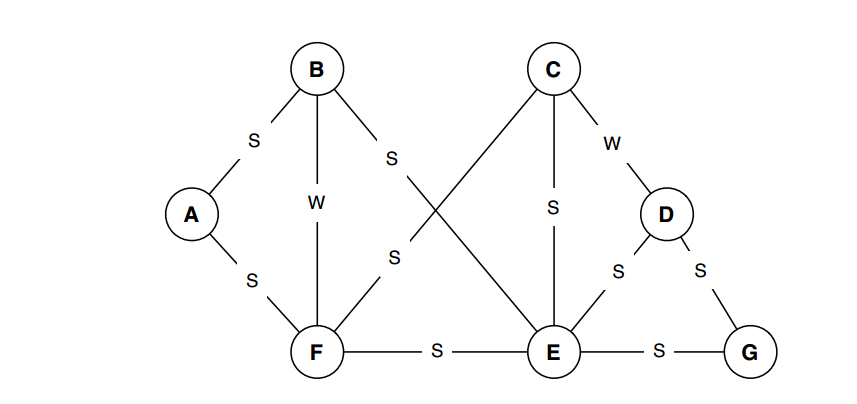
\includegraphics[width=15cm]{figures/figure1.png}
\caption{Une figure simple en \LaTeX. Issue de http://tinyurl.com/nqtrlj5.}
\label{fig:graph}
\end{figure}

\lipsum  % Remplacer avec votre texte

Voir \autoref{fig:graph}.


\section{Une section contenant un tableau}

\lipsum  % Remplacer avec votre texte

\begin{table}[ht]
\center
\begin{tabular}{cc|c}
A & B & A XOR B\\
\hline
0 & 0 & 0\\
0 & 1 & 1\\
1 & 0 & 1\\
1 & 1 & 0\\
\end{tabular}
\caption{Un tableau très simple en \LaTeX.}
\label{tab:xor}
\end{table}

\lipsum  % Remplacer avec votre texte

Cela est montré dans le \autoref{tab:xor}.


\section{Résumé}

\lipsum  % Remplacer avec votre texte
